% -------------------------------------------------------------------------------- %

\begin{exercise}[Exercise 4.1]

In Example 4.1, if $\pi$ is the equiprobable random policy, what is $q_\pi(11, \mathit{down})$?

\begin{center}
    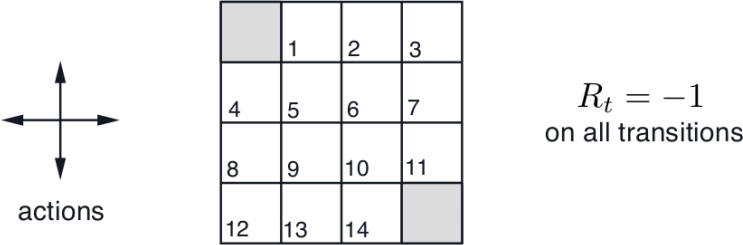
\includegraphics[width = 0.5 \textwidth]{2.22.png} \\
    Example 4.1
\end{center}

\end{exercise}

% -------------------------------------------------------------------------------- %

\begin{solution}

Let $\infty$ denote the lower right terminal state.
$v_\pi$ has already been calculated in Figure 4.1 from \cite*[page 77]{SuttonRichardS2018Rl:a}.
We only have to apply (4.6) from \cite*[page 78]{SuttonRichardS2018Rl:a}

\begin{align*}
    q_\pi(11, \mathit{down})
    & =
    \sum_{s^\prime, r}
        p(s^\prime, r \mid 11, \mathit{down})
        \bbraces{r + v_\pi(s^\prime)} \\
    & =
    p(\infty, -1 \mid 11, \mathit{down})
    \bbraces{-1 + v_\pi(\infty)} \\
    & =
    1 [-1 + 0] \\
    & =
    -1
\end{align*}

\end{solution}

% -------------------------------------------------------------------------------- %
